\documentclass[11pt]{amsbook}

\usepackage{../HBSuerDemir}


\begin{document}

    \hPage{b1p2/310}
    
    \begin{flushleft}
    side of $\ell$.
    \end{flushleft}

    \subsection*{D. CURVES} \hfill\\
    
    Circle and line are some curves having polar equations
    
    \begin{equation*}
         r=a,\ r=a\ cos\theta,\ r^2 -2r_{0}r cos(\theta-\theta_{0}) + r_{0}^2 -a^2=0
    \end{equation*}
    
    \begin{equation*}
        \theta = \theta_{0},\ r=a\ sec\theta,\ r(Acos\theta + Bsin\theta) + C =0
    \end{equation*}
    
    \hfill
    
    \begin{flushleft}
    which are in the form $r=f(\theta)$, or $F(\theta,r)=0$.
    \end{flushleft}
    
    \hfill
    
    An equation $r=f(\theta)$, $\theta=g(r)$ or $F(\theta,\ r)=0$ represents a curve in general, where $f$ may be a periodic function. \\
    
    \underline{Sketching:} \\
    
    A general procedure may be outlined as follows: \\
    
    1) \emph{Determination of the domain D} of $r=f(\theta)$ or of $F(\theta,r)=0$ \\
    
    If f is not periodic, vary $\theta$ in D.If f has period T, vary $\theta$ in $(0, T)$ and complete the curve by rotations through multiples of T about 0. \\
    
    2) \emph{Determination of symmetries} with respect to PA, CPA and the pole. \\
    
    If a symmetry exists the domain is reduced. Conditions for symmetries with respect to polar, copolar axes and the pole are given in following table:
    
    \begin{table}[ht]
        \begin{tabular}{c c c}
             \noindent\underline{\makebox[1.4in][l]{\hspace{13mm}PA}} & \noindent\underline{\makebox[1.4in][l]{\hspace{13mm}CPA}}  & \noindent\underline{\makebox[1.4in][l]{\hspace{13mm}Pole}} \\
             $F(-\theta,r)=F(\theta,r)$ & $F(-\theta,-r)=F(\theta,r)$ & $F(\theta,-r)=F(\theta,r)$ \\
             or & or &  or \\
             $F(\pi-\theta,-r)=F(\theta,r)$ & $F(\pi-\theta,r)=F(\theta,r)$ & $F(\theta+\pi,r)=F(\theta,r)$ \\
             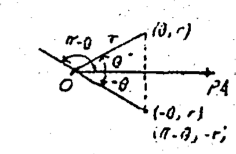
\includegraphics[width=1.4in]{images/b1p2-310-fig01.png} &
             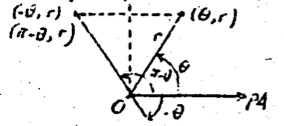
\includegraphics[width=1.4in]{images/b1p2-310-fig02.png} &
             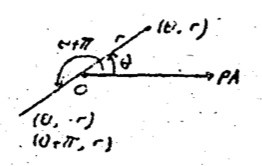
\includegraphics[width=1.4in]{images/b1p2-310-fig03.png}
        \end{tabular}
    \end{table}
    
\end{document}  